% !TeX spellcheck = ru_RU
% !TEX root = vkr.tex

\section{Обзор}
В этом разделе будут введены необходимые для понимания работы термины и  понятия.
\subsection{Деревья квадрантов}
Деревья квадрантов~--- рекурсивная структура данных для представления разряженных матриц. Данная матрица приводится до квадратной с размером, равным степени двойки, далее,если все элементы матрицы равны, то дерево представляется в виде пары значения и размера и будет называться листом дерева, в ином случае разделяется на четыре равные части~--- дочерние узлы (квадранты), которые тоже представляют собой деревья квадрантов. Так происходит до тех пор, пока каждый узел не дойдёт до листа. Таким образом, строится дерево в привычном для математиков понимания этого слова. визуальное представление этого процесса представлено на рис. \ref{qmatrix} и рис. \ref{qtree1}. Эта структура позволяет \enquote{сжимать} повторяющиеся и находящиеся близко данные в один узел.
\begin{figure}[ht]
    \centering
    % First minipage
    \begin{minipage}[b]{0.45\textwidth}
        \centering
        \resizebox{\linewidth}{!}{
            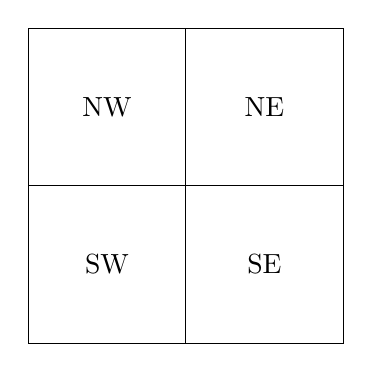
\begin{tikzpicture}
                \draw (1, 1) rectangle (3, 3);
                \draw (1, 3)rectangle (3, 5);
                \draw (3, 1)rectangle (5, 3);
                \draw (3, 3)rectangle (5, 5);
                \node at (2, 2){SW};
                \node at (4, 4){NE};
                \node at (2, 4){NW};
                \node at (4, 2){SE};
            \end{tikzpicture}
        }
        \caption{Квадратная матрица, разделенная на квадранты}
        \label{qmatrix}
    \end{minipage}
    \hfill
    % Second minipage
    \begin{minipage}[b]{0.45\textwidth}
        \centering
        \Tree [.Matrix
                [.NW [] ]
                [.NE [] ]
                [.SW [] ]
                [.SE [] ]
        ]
        \caption{Схематичное изображение одного из узлов дерева квадрантов и его потомков}
        \label{qtree1}
    \end{minipage}
\end{figure}

\subsection{Слияние ядер}
% Слияние ядер (англ. \textit{kernel fusion})
Требует уточнения
\subsection{Метапрограммирование}
Метапрограммирование~--- это процесс создание программ, которые в ходе своего выполнения генерируют другие программы. В контексте поставленной задачи оно было необходимо, так как нужно было
\begin{enumerate}[label=(\alph*)]
    \item генерировать функции в зависимости от данных, поданных пользователем;
    \item размер этого кода был довольно большим, но при этом обладал вполне регулярной структурой.
\end{enumerate}
В языке \Haskell{} есть встроенная библиотека с обширной и доступной документацией: \Th{}, которая позволяет генерировать код на \Haskell{} во время компиляции. При этом возможно использовать как синтаксис источника, так и более строгий специализированный для генерации кода.
